\documentclass[spanish, fleqn]{article}
\usepackage{babel}
\usepackage[utf8]{inputenc}
\usepackage{amsmath}
\usepackage{amsfonts}
\usepackage{mathrsfs}
\usepackage{dcolumn}
\usepackage[colorlinks, urlcolor=blue]{hyperref}
\usepackage{fourier}
\usepackage{tikz}
\usepackage{float}
\usetikzlibrary{arrows,shapes,snakes,automata,backgrounds,petri,babel,positioning}
\usepackage{pgf}
\usepackage[top = 2.5cm, bottom = 2cm, left = 2cm, right = 2cm]{geometry}
\definecolor{navyblue}{RGB}{0,148,222}
\definecolor{supercolor}{RGB}{0,148,12}
\tikzstyle{transition}=[rectangle,thick,draw=black!75,fill=black!20,minimum size=8mm]

\newcommand{\num}{1}

\title{INF-155: Introducción a la Informática Teórica\\
       ILI-225: Informática Teórica \\[0.4\baselineskip]
       Tarea \#\num \\
       \emph{``Este es el título de la tarea''}
      }
\author{\href{mailto:daniel.quinteros.12@sansano.usm.cl}{Daniel Quinteros}\\
20122012-2}
\date{6 de Abril 2017}

\begin{document}
\maketitle

\thispagestyle{empty}

\section*{Preguntas}

\begin{enumerate}

    \item Pregunta \(1\)
    \item Pregunta $2$
 
\end{enumerate}

\section*{Solución}
    
    \begin{enumerate}

        \item Solución a la primera pregunta.
        \item Un DFA puede ser:
        
        \begin{center}
        	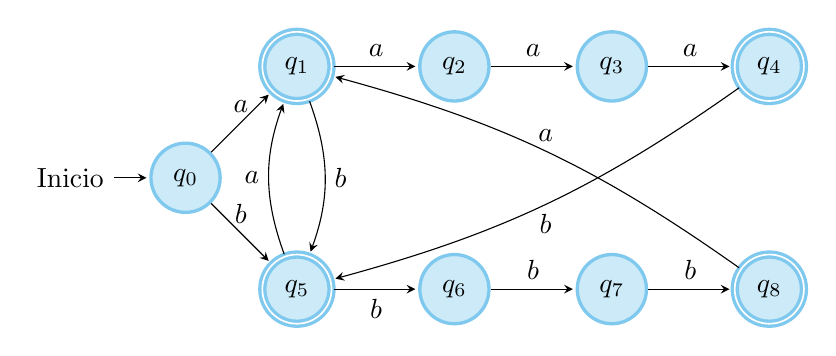
\begin{tikzpicture}[shorten >=1pt,node distance=2cm,on grid, >=stealth, initial text=Inicio, every state/.style={draw=navyblue!50,very thick,fill=navyblue!20}, bend angle=35]]
        		\node[state,initial]    (q_0)                        {$q_0$};
                \node[state,accepting]	(q_1) [above right of = q_0]   {$q_1$};
                \node[state]            (q_2) [right of = q_1]         {$q_2$};
                \node[state]            (q_3) [right of = q_2]         {$q_3$};
                \node[state,accepting]	(q_4) [right of = q_3]         {$q_4$};
        		\node[state,accepting]	(q_5) [below right of = q_0]   {$q_5$};
        		\node[state]            (q_6) [right of = q_5]         {$q_6$};
        		\node[state]            (q_7) [right of = q_6]         {$q_7$};
        		\node[state,accepting]	(q_8) [right of = q_7]         {$q_8$};
        	
            \path[->]   (q_0) edge node [above]                 {\(a\)} (q_1)
                        (q_0) edge node [above]                 {\(b\)} (q_5)
                        (q_1) edge node [above]                 {\(a\)} (q_2)
                        (q_2) edge node [above]                 {\(a\)} (q_3)
                        (q_3) edge node [above]                 {\(a\)} (q_4)
                        (q_4) edge[bend left=10] node [below]   {\(b\)} (q_5)
                        (q_5) edge node [below]                 {\(b\)} (q_6)
						(q_6) edge node [above]                 {\(b\)} (q_7)
						(q_7) edge node [above]                 {\(b\)} (q_8)
						(q_8) edge[bend right=10] node [above]  {\(a\)} (q_1)
						(q_1) edge[bend left=20] node [right]	{\(b\)} (q_5)
						(q_5) edge[bend left=20] node [left]    {\(a\)} (q_1);
        	\end{tikzpicture}
    	\end{center}
        
 
    \end{enumerate}

    
\end{document}